%% Elsevier / Journal of Systems and Software draft.
%% Template source: official Elsevier elsarticle package.
\documentclass[preprint,12pt,authoryear]{elsarticle}

\usepackage{amssymb}
\usepackage{amsmath}
\usepackage{booktabs}
\usepackage{array}
\usepackage{longtable}
\usepackage{tabularx}
\usepackage{xltabular}
\usepackage{makecell}
\usepackage{enumitem}
\usepackage[protrusion=true,expansion=false]{microtype}
\usepackage{xurl}
\usepackage{float}

\newcolumntype{Y}{>{\raggedright\arraybackslash}X}
\setlength{\emergencystretch}{3em}
\setlength{\bibsep}{0pt plus 0.2ex}

%% Float placement: keep full-width tables near their first mention instead of
%% deferring tall floats to the end of the document.
\renewcommand{\topfraction}{0.9}
\renewcommand{\bottomfraction}{0.8}
\renewcommand{\textfraction}{0.07}
\renewcommand{\floatpagefraction}{0.7}
\setcounter{topnumber}{3}
\setcounter{totalnumber}{5}

%% ---- Canonical two-layer MetaPattern model symbols (vendored from
%% P1-MetaPattern/shared/two_layer_canon.tex; single source of truth).
%% Term map: MR = metamorphic relation; MetaPattern = 元模式; MR family =
%% 蜕变关系族. Do not reintroduce "block" synonyms. ----
\providecommand{\AP}{\mathcal{A}_{P}}
\providecommand{\MM}{\mathbb{M}(\mathcal{A}_{P})}
\providecommand{\Grp}{G}
\providecommand{\Ord}{O_{\le}}
\providecommand{\Sadj}{T^{*}}
\providecommand{\Trev}{\mathcal{T}^{*}_{\mathrm{rev}}}
\providecommand{\Lim}{\mathcal{L}^{*}}
\providecommand{\minv}{m_{\mathrm{inv}}}
\providecommand{\mmono}{m_{\mathrm{mono}}}
\providecommand{\madj}{m_{\mathrm{adj}}}
\providecommand{\mrev}{m_{\mathrm{rev}}}
\providecommand{\mconv}{m_{\mathrm{conv}}}
%% L2 MR-family symbols (sans-serif f_{parent.child}), per two_layer_canon.tex.
\providecommand{\fIeqv}{\mathsf{f}_{\mathrm{inv}.\mathrm{eqv}}}
\providecommand{\fIcon}{\mathsf{f}_{\mathrm{inv}.\mathrm{con}}}
\providecommand{\fAself}{\mathsf{f}_{\mathrm{adj}.\mathrm{self}}}
\providecommand{\fAdual}{\mathsf{f}_{\mathrm{adj}.\mathrm{dual}}}
\providecommand{\fRtraj}{\mathsf{f}_{\mathrm{rev}.\mathrm{traj}}}
\providecommand{\fMstat}{\mathsf{f}_{\mathrm{mono}.\mathrm{stat}}}
\providecommand{\fMshape}{\mathsf{f}_{\mathrm{mono}.\mathrm{shape}}}
\providecommand{\fClim}{\mathsf{f}_{\mathrm{conv}.\mathrm{lim}}}
\providecommand{\fCrate}{\mathsf{f}_{\mathrm{conv}.\mathrm{rate}}}
\providecommand{\fCrepr}{\mathsf{f}_{\mathrm{conv}.\mathrm{repr}}}
\providecommand{\Translate}{\textsc{Translate}}

\journal{Journal of Systems and Software}

\begin{document}

\begin{frontmatter}

\title{Numerical-Decidability-Gated Metamorphic Testing for SciML Surrogates}

\author[inst1,inst2,inst3]{Meng Li\corref{cor1}\fnref{orcid-ml}}
\ead{mlemon@usc.edu.cn}
\author[inst1,inst2,inst3]{Xiaohua Yang\fnref{orcid-xy}}
\ead{xiaohua1963@foxmail.com}
\author[inst1,inst2,inst3]{Jie Liu\fnref{orcid-jl}}
\ead{jieliu@usc.edu.cn}
\author[inst1,inst2,inst3]{Shiyu Yan\fnref{orcid-sy}}
\ead{yanshiyu@usc.edu.cn}
\cortext[cor1]{Corresponding author: Meng Li.}
\fntext[orcid-ml]{ORCID: Meng Li, 0000-0002-1074-1502.}
\fntext[orcid-xy]{ORCID: Xiaohua Yang, 0000-0002-2977-1787.}
\fntext[orcid-jl]{ORCID: Jie Liu, 0009-0008-1970-8347.}
\fntext[orcid-sy]{ORCID: Shiyu Yan, 0000-0001-7626-5185.}
\affiliation[inst1]{organization={School of Computing, University of South China},
  city={Hengyang}, postcode={421001}, country={China}}
\affiliation[inst2]{organization={Hunan Engineering Research Center of Software Evaluation and Testing for Intellectual Equipment},
  city={Hengyang}, postcode={421001}, country={China}}
\affiliation[inst3]{organization={CNNC Key Laboratory on High Trusted Computing},
  city={Hengyang}, postcode={421001}, country={China}}

\begin{abstract}
Scientific machine-learning (SciML) surrogates are hard to test because exact
outputs are unavailable for transformed inputs. Metamorphic testing can
turn physical relations into oracle-free tests, but a candidate relation is not
automatically an interpretable verdict: a failure may reflect a surrogate
inconsistency, an invalid relation application, or a numerical artifact of the
measurement operator. This paper treats numerical decidability as a
SciML-specific admissibility condition for metamorphic testing. The novelty is
not that MR outcomes are recorded, but that a physics-derived relation is
admitted only when its physical basis, transformation preconditions,
representation mapping, and measurement-operator floor make a relation-level
verdict meaningful. The workflow executes admitted checks and retained stress
checks, but only admitted in-domain failures may support SUT-inconsistency
claims. For a P1
discrete-divergence check on shape-regular triangular meshes, we give a local
measurement-floor bound and instantiate it on the cylinder-flow mesh, with a
second Delaunay topology used as bounded stability evidence. The gate changes
verdicts rather than only annotating them: it defers absolute conservation when
the floor dominates, rejects an inadmissible airfoil continuity relation on
physical-basis grounds, and keeps node permutation as an implementation sanity
check. Bounded MeshGraphNets, PointMLP, PINN, FNO, airfoil, and cross-program
executions show that detector coverage follows the admitted relation set. The
evidence supports a SciML admissibility method, not general SciML reliability,
baseline superiority, arbitrary-mesh soundness, or real-world defect-detection
rates.
\end{abstract}

\begin{keyword}
Metamorphic testing \sep oracle problem \sep scientific machine learning \sep software testing \sep verification and validation
\end{keyword}

\end{frontmatter}

\section{Introduction}
\label{sec:introduction}

Scientific machine-learning (SciML) surrogates are increasingly used as software components for expensive simulations \citep{raissi2019pinn,karniadakis2021piml,li2021fno}. Mesh-based neural simulators such as MeshGraphNets (MGN) predict physical fields on irregular meshes \citep{pfaff2021meshgraphnets}, but for many transformed inputs there is no cheap exact output oracle \citep{barr2015oracle}. Held-out rollout error is necessary, yet it does not show whether a surrogate preserves relations that should hold under physically meaningful transformations.

Metamorphic testing (MT) addresses the oracle problem by checking relations across executions \citep{chen1998metamorphic,segura2016survey}. Conservation, symmetry, nondimensional similarity, and continuity can suggest candidate MRs for scientific software \citep{kanewala2019scientific,lin2020exploratory,olsen2019simulation}. This paper starts after candidates exist. A physics-derived relation is not automatically a valid software test: mirror symmetry may depend on geometry and boundary labels; divergence may depend on a discrete operator, mesh weights, and boundary treatment; and a transformed case may leave the relation's domain before revealing any system-under-test (SUT) inconsistency.

For SciML surrogate software, a failed MR check may indicate SUT inconsistency, invalid relation use, incompatible output mapping, or an unresolvable scoring floor. Treating all outcomes as ordinary pass/fail MT verdicts makes the evidence hard to audit and easy to overclaim.

Here, a candidate relation becomes an oracle-free test only when it is valid
for the SUT and measurable for the deployed discretization. The recording
workflow is conventional; the contribution is the SciML-specific decision rule
used before a failed relation check is reported as software evidence. A
downgraded relation may still be OOD stress evidence, but not a SUT fault
verdict. The evidence supports bounded SciML V\&V utility rather than general
reliability or real-world defect-detection rates.

\paragraph{Reader map.}
The method uses five concepts. A \emph{candidate relation} is a property the
SUT should preserve under a controlled change. A \emph{validity gate} asks
whether that relation is meaningful for this SUT and transformed case.
\emph{Numerical decidability} requires the metric and tolerance to distinguish
a real relation violation from the measuring operator's floor. An
\emph{executable check} runs the source/follow-up test built from an admitted
relation. A \emph{typed verdict} records pass, in-domain failure,
out-of-relation-domain, numerical deferral, or inconclusive evidence. All other terms in the paper are implementation details or evidence records built from these five concepts. In short, the paper screens a proposed relation, executes it only when valid and measurable, records a typed verdict, and restricts claims to that verdict.

Two principles organize the method. First, a relation is admitted only when its
validity conditions hold for the SUT and its tolerance dominates the measuring
operator's intrinsic floor. Second, relation outcomes are interpreted along
relation-violation and domain-violation axes, separating SUT inconsistency from
out-of-relation-domain use, numerical-floor deferral, and inconclusive evidence.
The main setting is MeshGraphNets-family cylinder flow, with the same predicate
exercised on a second CFD task and additional PDE families; these are bounded
case studies, not a completed applicability map.

\textbf{Contributions.} The paper contributes a SciML-specific
numerical-decidability gate for metamorphic testing. A physics-derived relation
is not admitted because it is plausible or recordable; it is admitted only when
its physical basis, transformation domain, representation mapping, and verdict
tolerance make the failure interpretable as relation-level software evidence.
The contribution is methodological, with domain-inadmissibility verdicts and
seeded-fault stress tests reported as stress evidence rather than validated
localization models.

\textbf{Numerical-decidability criterion.} For P1 constant-per-cell divergence on shape-regular triangular meshes and $C^2$ divergence-free reference fields, the operator floor is bounded locally by a mesh-shape constant times the Hessian scale and cell diameter. For the deployed cylinder-flow setting, this specializes to a tighter closed-form structured-mesh predictor that matches the measured floor to within 0.5\%, a rigorous a-priori bound that dominates it, and observed topology stability across a structured mesh and an unstructured Delaunay mesh (Sec.~\ref{subsec:operator-floor-sweep}); arbitrary degenerate or operator-mismatched meshes remain outside scope.

\textbf{Auditable implementation mechanism.} The gate is implemented through structured relation records and executable runners that record the transformation, mapping, metric, tolerance, exclusion rule, and ledger fields needed for independent inspection.

\textbf{Typed relation-level verdicts.} The verdict scheme is the gate's interpretation layer. It separates relation violation from domain violation, instantiating for physics-governed SciML the constraint-architecture pattern behind bug-versus-inapplicability reasoning \citep{duqueTorres2023bugornot,duqueTorres2023completePipeline} and MetaTrimmer \citep{duqueTorres2023metaTrimmer}. The added element is a typed classification of physical, geometric, boundary-condition, mapping, and operator-admissibility limits.

\textbf{Bounded necessity evidence.} The case studies evaluate what the criterion changes beyond rollout accuracy, generic MR generation, and LLM-assisted MR elicitation, using cylinder-flow runs plus airfoil, PINN, FNO, periodic-advection, RealPDEBench, a five-unit external issue/PR/commit-linked witness corpus, and cross-program checks. The evidence is complementarity and gate value, not baseline superiority or a general fault-detection-rate claim.

\section{Related Work}
\label{sec:related}

\subsection{Oracle-free testing and MR candidate sources}
\label{subsec:mesh-simulation}
\label{subsec:mt-oracle}
\label{subsec:mr-identification}

Mesh-based neural simulators learn dynamics on graph or mesh representations. MeshGraphNets encodes nodes and edges, propagates messages, and predicts future fields through autoregressive rollout \citep{pfaff2021meshgraphnets}. Here these models are software SUTs: a tester asks both whether rollout predictions are accurate and whether declared relations hold under controlled transformations and explicit tolerances.

MT checks relations among source and follow-up executions when per-input oracles are unavailable \citep{chen1998metamorphic,segura2016survey,chen2018mtSurvey}. It has been applied to scientific software, PDE programs, simulations, and ML systems \citep{chen2002pde,chen2011ml,kanewala2019scientific,olsen2019simulation}, including tabular credit scoring \citep{ying2025}. For SciML surrogates, however, an MR is not merely an input perturbation: validity depends on governing equations, boundary conditions, mesh representation, output mapping, and numerical tolerance. MR admissibility is therefore part of oracle construction.

Scientific-software MRs can be elicited from monotonicity, conservation, scaling, and domain-specific expectations \citep{kanewalaBieman2014slr,kanewala2019scientific,lin2020exploratory,olsen2019simulation,raunak2021continuum}. Candidate discovery has also used graph-kernel learning over source code \citep{kanewala2016graphkernel}, input/output-pattern separation and image-based output recognition for numerical solvers \citep{wang2022mridentification,fu2021burnup}, LLM-discovered variables \citep{tsigkanos2023}, statistical symmetry checks for trajectory predictors \citep{spieker2024trajectory,spieker2025multimodal}, data-driven transformations \citep{hiremath2021ocean}, and CPS design assumptions \citep{mandrioli2025cps}.

General MT tooling has explored machine-readable MR representations, constraint definition, test-data-driven MR selection, and specification languages \citep{duqueTorres2023completePipeline,duqueTorres2024selecting,sun2026ccml}. These systems strengthen MR engineering, but do not decide whether a physics-derived relation is numerically measurable, in-domain for a transformed CFD case, or interpretable as a SciML V\&V verdict.

These approaches supply candidate sources, but candidate identification is not admissible SciML test construction. MR identification, including our prior physics-derived MR construction for numerical solver and nuclear-power software \citep{li2022nuclearmr,wang2022mridentification}, is established work; this paper contributes the admissibility gate, not a new identification method. Fault-oriented work ranks MRs by detection power \citep{srinivasan2022prioritization,saha2019faultdetection}; here coverage is a bounded consequence of the admitted relation set.

\subsection{Physics-based MT, tolerance, and applicability}
\label{subsec:physics-mt}

Three contemporary strands are closest to this paper. Yang and Chui \citep{yang2021hydromt} and Reichert et al.~\citep{reichert2024hess} applied physics-derived MRs to hydrologic ML or conceptual models, showing that learned-model accuracy and relation consistency can diverge and that calibration or forcing regimes affect interpretation. Eniser et al.~\citep{eniser2022relaxations} introduced \emph{relaxations}, numerical tolerances embedded in MR oracles, for stochastic reinforcement-learning (RL) policy testing. Duque-Torres et al.~\citep{duqueTorres2023bugornot,duqueTorres2023completePipeline,duqueTorres2024selecting} and MetaTrimmer \citep{duqueTorres2023metaTrimmer} address bug-versus-inapplicability reasoning with explicit MR constraints and automated constraint derivation.

The present work combines relation-level physics checks, calibrated tolerances, and bug-versus-inapplicability reasoning. Its added condition is numerical decidability: the verdict tolerance must dominate the measuring operator's intrinsic error floor, a discretization property fixed before any fault or SUT is considered. The floor gate, not the recording discipline, is the new element. The admissibility decision, tolerance rationale, executable check, and typed verdict are then recorded together and tied to evidence artifacts. Table~\ref{tab:closest-prior-positioning} positions the paper against the closest-prior capabilities.

\begin{table}[H]
\centering\footnotesize
\caption{Closest-prior capability matrix.}
\label{tab:closest-prior-positioning}
\renewcommand{\arraystretch}{0.82}
\begin{tabularx}{\textwidth}{@{}>{\raggedright\arraybackslash}p{0.22\textwidth}YYY@{}}
\toprule
Approach & What it supplies & What remains missing for the evaluation objective & What this paper adds \\
\midrule
Scientific-software MR identification & Candidate relations from domain rules, source-code learning, LLM variables, and data-driven search & Candidate validity, numerical decidability, executable check format, and typed SciML verdicts & Treats these methods as candidate sources, not validity authorities \\
Reichert et al. & Physics-derived MRs and informal filtering in a learned hydrologic surrogate & Explicit admissibility predicate, operator-floor tolerance, reusable relation records, and typed verdicts & Formalizes the candidate-to-verdict path for mesh-based SciML surrogates \\
Eniser et al. & Relaxed MR oracles with numerical thresholds & Measurement-operator floor and relation-domain interpretation for deterministic SciML surrogates & Grounds tolerance in the scoring operator's own numerical floor \\
Duque-Torres / MetaTrimmer & Binary bug-versus-inapplicability separation with explicit MR constraints and automated constraint derivation & A typed inadmissibility verdict and operator-floor admissibility for physics-governed SciML & Replaces the binary skip/proceed pre-filter with a two-axis typed verdict tied to physical, geometric, boundary, and operator limits \\
Formal MR specification and constraint tooling & Machine-readable MR descriptions, constraint phases, and supporting systems & Physics-specific admissibility dimensions, measurement floors, and executable evidence ledgers for SciML & Uses specification ideas but binds each verdict to relation-domain and numerical-decidability evidence \\
\textbf{This paper} & Physics, expert, and LLM-assisted candidates plus artifact-backed execution & Bounded case-study evidence, not general SciML reliability or baseline superiority & Constructs relation records, runners, ledgers, and typed verdicts under a four-condition gate \\
\bottomrule
\end{tabularx}
\end{table}

\subsection{SciML diagnostics and positioning}
\label{subsec:sciml-vv}
\label{subsec:hybrid-trust}
\label{subsec:new-not-new}

SciML reliability tools include physics residuals, uncertainty quantification (UQ), conformal prediction, certified error bounds, and failure-mode analysis \citep{raissi2019pinn,karniadakis2021piml,li2021fno,krishnapriyan2021failure,gopakumar2025calibrated}. PINN gradient-flow pathologies \citep{wang2021gradflow,krishnapriyan2021failure} sharpen the need for checks that do not assume a converged surrogate. These diagnostics are not competitors to MT: a residual, equivariance error, or uncertainty score becomes an executable MR only when paired with a source case, follow-up transformation, tolerance rule, exclusion rule, and verdict interpretation.

Hybrid ML-solver frameworks use residual thresholds or error estimates to decide when a learned component should be trusted \citep{baral2025xrepit,wang2025deeponetfe}. Such systems operationalize runtime trust regions, whereas this study acts offline, applying physically derived transformations before deployment to estimate where relation violations occur.

The distinction from residual- and uncertainty-based trust estimation is deliberate. UQ, conformal prediction, residual thresholds, and physical-consistency diagnostics score observed outputs \citep{najafi2026}; this method acts in relation space, applying a controlled transformation and reporting which necessary relation breaks under it. The claim is complementarity, not superiority.

Metamorphic testing, MR identification, scientific-software MT, residual diagnostics, uncertainty quantification, LLM candidate generation, and the NOETHER two-layer MetaPattern model are established or emerging sources of testing ideas. The contribution here is narrower: SciML MR use should be treated as a numerical-decidability problem before it is treated as a test-execution problem. A candidate relation becomes useful only after its physical basis, transformation domain, representation mapping, and measurement floor make a relation-level verdict interpretable. Recent work derives or refines domain-specific MRs for scientific programs directly from their numerical models \citep{yan2024elliptic,stevens2025mars}; the wedge here is the learned surrogate evaluated out of distribution and the requirement that a relation's tolerance dominate the measuring operator's numerical floor, rather than testing a numerical solver against derived relations. The missing combination is thus a SciML-specific admissibility gate whose executable records make the decision auditable (Table~\ref{tab:closest-prior-positioning}).

\section{Method}
\label{sec:method}

\subsection{Overview}
\label{subsec:method-overview}

The method turns a physics-derived candidate relation into relation-level
software evidence only after three checks are made explicit: validity gating,
executable-check construction, and verdict interpretation. The executable
records are the audit trail, not the main novelty. The central decision is
SciML-specific: expert reasoning, physical laws, the NOETHER two-layer
MetaPattern model, and LLM-assisted lists may propose relations, but none
certifies that a relation is physically valid, representation-compatible, and
numerically measurable for a specific SUT.

\textbf{Formal spine.} Let \(r=(b,T,M,m,\tau,P)\) denote a candidate relation, where \(b\) is its basis, \(T\) the source-to-follow-up transformation, \(M\) the output mapping, \(m\) the metric, \(\tau\) the tolerance, and \(P\) the preconditions. For SUT \(s\) and source case \(x\), the gate returns \(G(r,s,x)\in\{\mathrm{admit},\mathrm{reject},\mathrm{stress},\mathrm{defer}\}\). If admitted or retained as stress evidence, execution returns \(E(r,s,x)=(y,y',z)\), where \(y\) and \(y'\) are source and follow-up outputs and \(z\) is the measured relation evidence. The verdict map \(V(G,z)\) assigns the typed verdict. Only an admitted relation with a fail verdict inside the relation domain can support a SUT-inconsistency claim.

\textbf{Terminology and verdict types.} A verdict is read on two axes, relation-violation and domain-violation magnitude (detailed in Sec.~\ref{subsec:verdicts}). A candidate relation is accordingly \emph{admitted} (a large in-domain violation reads as SUT inconsistency), \emph{rejected} on physical grounds, \emph{deferred} when no tolerance dominates the operator floor, \emph{out-of-relation-domain}, or \emph{inconclusive}. Four MR families recur in the case studies: node-permutation equivariance, mirror-y reflection symmetry, discrete-divergence continuity/conservation, and exact mirror-y on a constructed symmetric mesh. As a running example, a mirror-y candidate is first checked against geometry and boundary labels; on an asymmetric mesh it becomes OOD stress rather than a fault oracle, while on a constructed symmetric mesh it remains an admitted equivariance test.

\begin{figure}[!htbp]
\centering

\includegraphics[width=0.85\linewidth]{figures/fig_1_validity_gated_workflow.pdf}
\caption{Admissibility-gated V\&V workflow.}
\label{fig:workflow}
\end{figure}

\subsection{Candidate relation sources and organization}
\label{subsec:candidate-sources}

This paper applies two prior MR-identification results rather than redefining MR identification. The four-layer classification of scientific-computing MRs \citep{yang2020hierarchical} asks where relations come from: physical, computational, code, or data layers. Its physical, computational, and code layers can yield real MRs when the corresponding semantic constraint is established. The two-layer MetaPattern model of NOETHER \citep{zhao2026noether}, a same-author preprint, asks a different question: what algebraic shape a candidate relation has. We use these two results to source and organize candidate relations, and use NOETHER only as an optional scaffold for generating and naming likely MR candidates. The central decision point in this paper is therefore not candidate discovery itself but the admissibility gate of Section~\ref{subsec:admissibility-gate}, which decides whether any candidate becomes an admissible MR for a specific SUT.

\emph{Layer~1 (MetaPattern).} A \emph{MetaPattern} is the equivalence class of MRs generated, through \Translate, from one minimal algebraic structure of the program-induced operator algebra $\AP$. The five MetaPatterns are generated by a group action ($\Grp$), partial order ($\Ord$), self-adjoint operator ($\Sadj$), time-reversal involution ($\Trev$), or parametrized limit ($\Lim$); their set is $\MM$. Conservation is therefore the group-action member $\minv$.

\emph{Layer~2 (MR family).} An \emph{MR family} instantiates one MetaPattern under a fixed transformation template and mode. Families use the form $\mathsf{f}_{\mathrm{parent}.\mathrm{child}}$; legacy letters a--j remain cross-reference anchors. The map is one-to-many: $\Grp \to \{\fIeqv, \fIcon\}$, $\Sadj \to \{\fAself, \fAdual\}$, $\Trev \to \{\fRtraj\}$, $\Ord \to \{\fMstat, \fMshape\}$, and $\Lim \to \{\fClim, \fCrate, \fCrepr\}$.

For the cylinder-flow surrogates studied here, the instantiated families are $\fIeqv$ (equivariance, a), mirror-y reflection; $\fIcon$ (conservation, b), discrete-divergence continuity and, on the airfoil task, compressible mass balance; $\fCrepr$ (representation-invariance, j), node-permutation and encoding contracts; and $\fClim$ and $\fCrate$ (convergence, accuracy-order, h--i), the operator-floor mesh-refinement relation. The $\fMstat$ (static-order, f) Reynolds--Strouhal monotonicity is a candidate not exercised here, $\fRtraj$ (trajectory-reversal, e) is empty by construction for viscous dissipative flow, and the self-adjoint families $\fAself$ and $\fAdual$ (c--d) appear only in the cross-family PINN and FNO extensions. The same relation may be admissible as one family yet inadmissible once instantiated for a given SUT: mirror symmetry holds on a symmetric domain but not on an asymmetric mesh with incompatible boundary labels, and conservation is a physical expectation but not an executable verdict when the discrete measuring operator has an unresolved floor. The admissibility gate records where each relation survives.

\subsection{Admissibility gate}
\label{subsec:admissibility-gate}

A candidate relation is an \emph{admissible MR} only when four conditions hold together. First, it must have a physical or software basis. Second, its transformation preconditions must hold for the source and follow-up cases. Third, boundary conditions and output mappings must remain compatible after transformation. Fourth, the verdict must be numerically decidable: the tolerance must dominate the intrinsic error floor of the measuring operator. None of these conditions is optional. Table~\ref{tab:admissibility-gate} records the gate, the Relation-record fields, and the verdict semantics.

\begin{table}[H]
\centering
\caption{Admissibility gate and verdict semantics.}
\label{tab:admissibility-gate}
\footnotesize
\renewcommand{\arraystretch}{0.92}
\setlength{\tabcolsep}{3pt}
\begin{tabularx}{\textwidth}{@{}>{\raggedright\arraybackslash}p{0.18\textwidth}>{\raggedright\arraybackslash}p{0.31\textwidth}>{\raggedright\arraybackslash}p{0.29\textwidth}Y@{}}
\toprule
\textbf{Method element} & \textbf{Required record} & \textbf{Allowed interpretation} & \textbf{Design role} \\
\midrule
Basis & Equation, boundary condition, nondimensional law, representation property, numerical assumption, or implementation contract & Relation may be considered only for SUTs where this basis applies & Gate \\
Preconditions & Source-case constraints, follow-up transformation, preserved quantities, and exclusion rule & Missing preconditions produce skip or out-of-relation-domain, not SUT failure & Gate \\
Mapping compatibility & Boundary-label compatibility and output mapping from follow-up output back to source coordinates/fields & Incompatible mapping rejects or downgrades the candidate & Gate \\
Numerical decidability & Metric, tolerance, tolerance provenance, and measurement-floor evidence & A verdict is meaningful only when tolerance dominates the operator floor & Gate \\
Relation record & Identifier, source category, transformation, mapping, metric, tolerance, exclusions, expected verdicts, and artifact schema & The admitted relation becomes a reusable executable V\&V check & Check \\
Ledger & Source/follow-up run ids, metric outputs, floor evidence, exclusions, logs, and verdict & The reported claim is auditable from artifacts rather than prose alone & Ledger \\
Verdict semantics & Pass, fail, skip, out-of-relation-domain, numerical-tolerance issue, or inconclusive & Only fail inside the valid domain may be read as SUT inconsistency & Verdict \\
\bottomrule
\end{tabularx}
\end{table}

The gate produces four design-time decisions: admit as an executable MR; downgrade to OOD-stress when the relation is physically informative but outside its exact domain; reject when basis, preconditions, or mapping fail; or defer when missing numerical evidence prevents a verdict. For example, node permutation can be admitted as a representation MR when the adapter and inverse mapping are deterministic; mirror-y is conditional on compatible geometry, boundary labels, and vector-component mapping; absolute discrete divergence is deferred when the reference field and measuring operator floor cannot support an absolute verdict.

\subsection{relation record and executable check format}
\label{subsec:relation-record}

A retained MR is represented as a structured relation record containing the fields listed in Table~\ref{tab:admissibility-gate}: identifier, source category, physical or software basis, source-case schema, follow-up transformation, preconditions, boundary-condition compatibility, output mapping, metric, tolerance and provenance, expected verdict classes, exclusion rules, artifact schema, and interpretation limits. The relation record is the reusable design record; the executable check operationalizes it.

Each executable check includes transformation code, runner configuration, metric computation, verdict logic, and artifact recording. The ledger is part of the method rather than only replication packaging: every relation-level claim must be traceable to the source run, follow-up run, mapping, metric output, floor evidence, exclusion decision, and verdict.

\subsection{Relation-level verdicts}
\label{subsec:verdicts}

An MR execution can produce: \textbf{pass} (relation holds within tolerance); \textbf{fail} (violated within the valid relation domain); \textbf{skip} (required precondition missing); \textbf{out-of-relation-domain} (the transformed case is outside the relation domain); \textbf{numerical-tolerance issue} (the measured effect is dominated by threshold or resolution uncertainty); or \textbf{inconclusive} (insufficient artifact).

These verdicts form the two-dimensional space in Figure~\ref{fig:verdict-2d}. One axis is relation-violation magnitude, typically expressed as a violation-to-floor or violation-to-tolerance ratio. The other is domain-violation magnitude: how far the transformed case lies outside the relation's validity domain. Low domain violation with high relation violation is the region that may be read as SUT inconsistency; high domain violation is out-of-relation-domain; a violation inside the error floor is a numerical-tolerance issue. This decomposition defines the method's verdict-interpretation role, which is evaluated explicitly in Section~\ref{subsec:rqs}.

In this study, the domain-violation coordinate is operationalized per relation from committed measurements. For mirror-y, $D = m/(m+1)$, where $m$ is the worst reflected-node placement error in median-edge-length units. The synthetic symmetric mesh scores $D \approx 0$, whereas the real asymmetric evaluation mesh scores $D = 0.51$. Other MR families use their own precondition measurements. These $D$ values denote structural placement within each relation's own validity domain: $D$ is a per-relation normalized coordinate, not a cross-relation calibrated metric, and the values cannot be averaged or ranked across MR families; read per relation, not as a calibrated boundary measurement. A cross-relation calibration would need to normalize each family by its own admissibility boundary, mapping every gate threshold to a common $D_{\mathrm{cal}} = 1$; that calibration is future work.

\begin{figure}[!htbp]
\centering
\makebox[\linewidth][c]{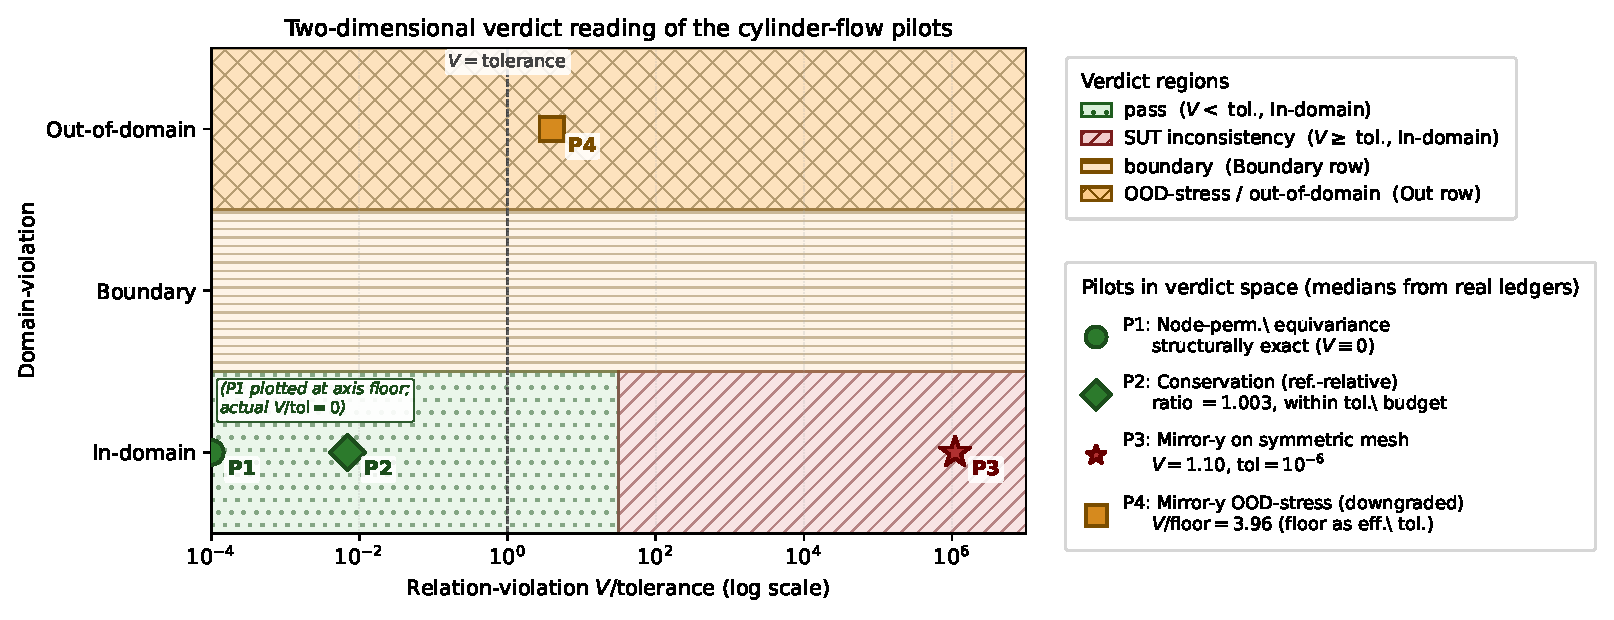
\includegraphics[width=1.08\linewidth]{figures/fig_3_verdict_2d.pdf}}
\caption{Two-dimensional relation and domain verdict space.}
\label{fig:verdict-2d}
\end{figure}

Retained MRs are interpreted through their two-layer position (Sec.~\ref{subsec:candidate-sources}): a relation's MetaPattern and MR family fix which algebraic invariant it measures, and therefore which faults it can and cannot surface. This is an interpretation protocol, not a validated localization model; the seeded-fault results later are a bounded stress test of it.

\paragraph{Practitioner checklist and adoption boundary.}
For a new SUT: (1) state the relation and source; (2) record source/follow-up preconditions; (3) check boundary labels and output mapping; (4) bound or calibrate the operator floor; (5) compare verdict tolerance with that floor; and (6) issue a typed verdict and ledger the run. The method does not remove domain expertise or automate MR discovery. Adoption costs are relation-specific physics review, mapping code, floor evidence, and bookkeeping; when any item is missing, the outcome is reject, defer, or OOD-stress, without a fault claim.

\section{Experimental Design}
\label{sec:empirical-design}

\subsection{Research questions}
\label{subsec:rqs}
\label{subsec:evaluation-logic}

The objective is to test whether physics-derived MRs for SciML surrogate software can become auditable oracle-free V\&V checks that distinguish SUT inconsistency from relation invalidity and numerical measurement limits, not population-wide defect-detection effectiveness.

This objective is decomposed into four research questions:
\begin{description}[leftmargin=!,labelwidth=2.4cm]
\item[RQ1 -- Screen.] Which validity conditions screen a physics-derived candidate MR before it is used as an oracle-free test for a specific SciML surrogate SUT?
\item[RQ2 -- Build.] How can admitted relations build reusable executable checks with explicit transformations, mappings, metrics, tolerances, exclusions, and evidence records?
\item[RQ3 -- Interpret.] How can typed verdicts interpret relation-level outcomes so that SUT inconsistency is separated from out-of-relation-domain application, numerical tolerance limits, and inconclusive evidence?
\item[RQ4 -- Evaluate.] In bounded SciML surrogate case studies, what evidence can evaluate the admissibility-gated workflow beyond rollout accuracy, generic MR generation, and LLM-assisted candidate elicitation?
\end{description}

\subsection{Experimental subjects}
\label{subsec:suts}

Subjects are selected for evidence roles, not statistical representativeness: a primary SciML surrogate setting, a changed physical task or architecture, a cross-family PDE/neural-operator setting, or a bounded defect/coverage witness. We do not sample by repository popularity, LOC, or issue-mined defects; that would be a separate real-defect study.

The executable inventory comprises two CFD tasks, same-task MGN variants, PointMLP, PhysicsNeMo, PINN/FNO rosters over two PDEs, one periodic-advection workflow, and five external CPU-only replays. Fault evidence comprises 10 canonical and two adversarial MGN mutants, 48 PINN/FNO probes, a PointMLP 20-fault catalogue, and the sibling's 70 witness rows plus 20 true-fault-class rows. These are scope denominators, not sampling frames for a defect-detection rate.

\begin{table}[!htbp]
\centering
\caption{Subject selection and evidence scope.}
\label{tab:subject-scope}
\scriptsize
\renewcommand{\arraystretch}{0.9}
\setlength{\tabcolsep}{3pt}
\begin{tabularx}{\linewidth}{@{}>{\raggedright\arraybackslash}p{0.20\linewidth}>{\raggedright\arraybackslash}p{0.45\linewidth}Y@{}}
\toprule
\textbf{Evidence block} & \textbf{Subjects and evidence role} & \textbf{Boundary} \\
\midrule
Cylinder-flow mesh surrogates & Primary executable workflow plus same-task implementation checks: MGN K=6 roster over three trajectories, S4/S5 variants, PointMLP, and PhysicsNeMo \texttt{MeshGraphNet}; seeded-fault stress uses 10 canonical MGN mutants, two adversarial mutants, and PointMLP 20-fault catalogue & Same task and bounded rosters; no real-defect rate or LOC-based representativeness \\
Airfoil mesh surrogate & Changed-physics gate discrimination on official DeepMind airfoil with PhysicsNeMo \texttt{MeshGraphNet}, K=6 checkpoints over 40 test trajectories & Typed inadmissibility evidence, not SOTA airfoil accuracy or official-checkpoint evidence \\
PINN/FNO and periodic PDE workflows & Cross-family PINN/FNO Burgers/heat predicate checks plus independent periodic-advection primary workflow with six periodic-convolution SUTs and 60 relation cells per admitted MR & Synthetic/generated PDE evidence; not production CFD, real-defect, reliability, or broad neural-operator claims \\
External witnesses & RealPDEBench foil preflight witness, five-unit external issue/PR/commit-linked witness corpus (including the DeepXDE PeriodicBC issue-linked witness, NeuralOperator, PhiFlow/PhiML, and JAX-CFD), and Minimum-MR-SubSet audit/replays & Triangulates outside the self-made cylinder setting; not production-CFD validation, trained-SUT correctness, or a representative defect-rate corpus \\
\bottomrule
\end{tabularx}
\end{table}

The evidence tiers are: \emph{primary} full-chain cylinder-flow and periodic-advection workflows; \emph{supporting} airfoil, PINN, and FNO gate checks; \emph{secondary} rollout, LLM/generic-candidate, RealPDEBench, external-witness, and sibling-rerun contrasts; and \emph{stress-test} seeded-fault and cross-program checks. The unit is a relation-level cell: relation record, SUT/checkpoint, source, follow-up, metric, and verdict. Effective-N and inference permissions are in the supplement; repeated cells remain descriptive evidence, not population samples.

\subsection{Evaluation metrics}
\label{subsec:metrics}

Primary metrics are admissibility decision, executable MR rate, verdict distribution, violation magnitude relative to tolerance or floor, exclusion rate, and relation-level interpretation. Secondary metrics include screening agreement, flakiness, complementarity with rollout accuracy, and seeded-fault detection by class. All are read at the relation-cell level, not as reliability or defect-rate estimates.

\subsection{Experimental method}
\label{subsec:experimental-method}

The experiments instantiate the candidate-to-check workflow of Section~\ref{sec:method}. Cylinder-flow relations cover equivariance ($\fIeqv$), conservation ($\fIcon$), representation-invariance ($\fCrepr$), and convergence/accuracy-order ($\fClim$, $\fCrate$); static-order and self-adjoint families appear only as candidate or cross-family checks, and trajectory-reversal is empty for viscous flow. Each retained relation records a relation record, source/follow-up executions, mapping artifacts, metric outputs, floor evidence, exclusions, and a typed verdict.

\subsection{Comparison baselines}
\label{subsec:baselines}

Rollout accuracy, residual/UQ diagnostics, expert-designed candidates, generic MR generators, and LLM-assisted candidates contextualize RQ4. Accuracy asks whether a prediction matches held-out data; an MR asks whether a declared relation holds under a controlled transformation. The contrast is complementarity and gate value--false-alarm removal, typed triage, auditability, and executable-check reuse--not superiority in a shared score. The gate, not the generator, decides whether a candidate becomes executable.

\subsection{Analysis plan and evidence mapping}
\label{subsec:rq-evidence}

Table~\ref{tab:rqmap} maps research questions to evaluation evidence, artifacts, units of analysis, and claim boundaries; it is a design rather than a result table.

\begin{table}[H]
\centering
\caption{Evaluation design.}
\label{tab:rqmap}
\scriptsize
\setlength{\tabcolsep}{1.5pt}
\begin{tabularx}{\linewidth}{@{}>{\raggedright\arraybackslash}p{0.08\linewidth}>{\raggedright\arraybackslash}p{0.22\linewidth}>{\raggedright\arraybackslash}p{0.20\linewidth}>{\raggedright\arraybackslash}p{0.21\linewidth}Y@{}}
\toprule
\textbf{Item} & \textbf{Evaluation question} & \textbf{Evidence tier and unit} & \textbf{Artifacts} & \textbf{Claim boundary} \\
\midrule
Goal & Does the full workflow connect candidate, gate, executable check, verdict, and evidence? & Primary workflow trace; Relation-record cell & relation records, runners, claim ledger & Records and checks only; no general reliability claim \\
RQ1 & Which candidates are admissible, rejected, downgraded, or deferred? & Primary and supporting gates; candidate/MR & Gate records, operator-floor sweep, exclusions & Physical validity is relation- and SUT-specific \\
RQ2 & Are admitted relations executable and auditable? & Primary execution cells; source/follow-up pair & Transformations, runner configs, metric files, logs & Execution completeness, not complete automation of MR discovery \\
RQ3 & Do verdicts separate SUT inconsistency from domain and numerical limits? & Verdict ledger; MR-by-case cell & Two-axis verdicts, metric/floor ratios, exclusion logs & Per-relation interpretation; no cross-relation calibrated domain score \\
RQ4 & What evidence is added beyond rollout accuracy and candidate-generation comparators? & Primary, supporting, secondary, and stress-test tiers & Rollout diagnostics, LLM/generic baselines, witness reruns, seeded-fault ledgers & Complementarity and bounded utility; no baseline superiority \\
Impl. & What blind spots follow from the admitted MR set? & Stress-test tier; mutant/MR cell & Seeded-fault catalogue and cross-SUT removal check & Bounded coverage interpretation, not real-world detection rate \\
\bottomrule
\end{tabularx}
\end{table}

The study reports inferential statistics only where the sampling structure supports them, labeling descriptive counts otherwise. Binary detector outcomes over the unified fault catalogue carry Wilson 95\% confidence intervals (CIs) per detector; continuous violation magnitudes use exact Wilcoxon signed-rank tests with a rank-based effect size (Cliff's $\delta$), where the design supports paired comparison; roster medians carry paired bootstrap intervals; and the operator-floor sweep reports a log-log slope with a 95\% CI. Repeated cells from one trajectory or one checkpoint family are reported as descriptive cell summaries, not independent population samples.

\subsection{Ethics, integrity, and reproducibility}
\label{subsec:ethics}

The study does not involve human subjects or personal data. SUT versions, datasets, checkpoints, scripts, and run logs are recorded when licensing permits. Failed, skipped, out-of-relation-domain, numerical-tolerance, and inconclusive outcomes remain in the ledger. LLM use is restricted to candidate generation and evidence organization, not validity judgment. No candidate MR is described as valid without a passing gate decision and relation record; no OOD violation is described as a program fault without supporting verdict evidence.

\section{Results and Discussion}
\label{sec:results}

Evidence is reported by research question rather than chronology (Table~\ref{tab:rqmap}). Roles keep breadth from becoming representativeness: cylinder-flow and periodic-advection are bounded primary full-chain workflows; airfoil, PINN, and FNO are supporting falsification checks; LLM/generic baselines and sibling reruns are secondary contrasts; and seeded faults stress detector blind spots. Baseline contrasts measure gate value, not method superiority.

\subsection{Evidence overview}
\label{subsec:claim-evidence-map}

The compact claim-to-evidence map binds claims to tracked artifacts; the full table is supplementary, and \texttt{claim-ledger.yml} remains authoritative.

\label{subsec:relation-record-verdict-map}

Table~\ref{tab:relation-record-verdict} is a compact verdict index; read each row as the same chain--candidate relation, gate decision, runtime verdict, and claim boundary--rather than as an independent population sample. Detailed paths and per-run artifacts are supplementary and ledgered.

{
\scriptsize
\renewcommand{\arraystretch}{0.92}
\setlength{\tabcolsep}{2.5pt}
\begin{xltabular}{\linewidth}{@{}>{\raggedright\arraybackslash}p{0.18\linewidth}>{\raggedright\arraybackslash}p{0.24\linewidth}>{\raggedright\arraybackslash}p{0.28\linewidth}Y@{}}
\caption{Relation-record verdict map.}\label{tab:relation-record-verdict}\\
\toprule
\textbf{Evidence block} & \textbf{Gate outcome} & \textbf{Runtime verdict} & \textbf{Boundary} \\
\midrule
Cylinder-flow MGN/variants & Node permutation admitted; mirror exact relation downgraded or admitted only on symmetric mesh; absolute conservation deferred & Node permutation exact; mirror OOD stress fails 180/180; exact symmetric-mesh mirror fails 18/18; reference-relative conservation passes 162/162 & Primary bounded workflow; absolute conservation remains deferred; no geometry-independent or population rate \\
Same-task architecture checks & Same predicate applied to S4/S5, PointMLP, and PhysicsNeMo cylinder executions & S4/S5 and PointMLP reproduce typed verdict pattern; PhysicsNeMo smoke records node-permutation pass and mirror OOD stress & Implementation artifact check, not production-scale reliability \\
Airfoil changed-physics task & Node permutation admitted; incompressible continuity and mirror-y rejected/deferred for physical/numerical reasons & 240/240 node-permutation exact; continuity and mirror verdict types change with compressible/non-zero-angle physics & Gate discrimination, not SOTA airfoil accuracy \\
FNO primary workflow upgrade & Translation admitted; periodic discrete-conservation admitted-with-reference-floor; Dirichlet translation rejected & 24/24 translation passes, 24/24 conservation failures, and 6/6 rejected Dirichlet exact-MR executions & Full gate-to-verdict FNO evidence, outside cylinder-flow and broad neural-operator claims \\
Periodic-advection primary workflow & Periodic translation and mass/mean conservation admitted; fixed-velocity mirror candidate rejected & 60/60 translation passes, 60/60 mass-conservation passes, and 6/6 fixed-velocity mirror rejections & Independent synthetic PDE workflow; not production CFD or real-defect evidence \\
External defect-witness corpus & Five documented external issue/PR/commit semantic contrasts admitted at component/utility level & 5/5 typed pass: DeepXDE derivative periodicity, NeuralOperator spectrum and Hermitian fixes, PhiML gradient axis order, JAX-CFD flux boundary & Stronger external-validity witness set; not representative defect sampling, trained-SUT correctness, production validation, or a defect rate \\
\bottomrule
\end{xltabular}
}

\subsection{Primary cylinder-flow evidence}
\label{subsec:within-sut-pilot}

All pilots use one trained MeshGraphNets cylinder-flow surrogate from the read-only Minimum-MR-SubSet checkpoint. They exercise three gate outcomes, with raw outputs, manifests, and metric ledgers mapped in the supplementary table.

The primary cylinder workflow has six readings: node permutation is an exact representation sanity check; asymmetric mirror-y is downgraded to OOD-stress and fails on 10/10 frames; absolute continuity is deferred while the reference-relative diagnostic is an \emph{inconclusive: reference-relative non-regression guard}; rollout accuracy answers a different question; exact mirror-y fails only after a symmetric mesh makes the relation admissible; and seeded faults show MR-family-specific blind spots.

\textbf{Representation MR.} Node-permutation equivariance holds to machine precision (relative L2 = 0.0 at tolerance 1e-6), a pipeline sanity check rather than model-capability evidence.

\textbf{Geometric MR.} Exact mirror-y is out-of-relation-domain on the asymmetric mesh: reflection is non-bijective, the worst reflected-node mismatch is about one edge length, and the cylinder is off-centre by 7.2 mm. The downgraded nearest-neighbour OOD-stress probe \textbf{failed on 10 of 10 recorded eval frames} (median relative L2 0.737, median V/floor 3.96), with no skipped or inconclusive frame. This is descriptive evidence from one SUT, checkpoint, MR, and trajectory; the symmetric-mesh run tests whether the failure is only geometric.

\textbf{Continuity MR.} The P1 discrete-divergence operator gives non-negligible divergence even on ground truth, so absolute mass conservation is deferred. Predicted divergence stays within about 0.4--0.8\% of the reference, with an interior-only check against a pure boundary artifact. Because the reference term is not decomposed into operator error, solver artifact, or non-solenoidal data, the verdict is \emph{inconclusive: reference-relative non-regression guard}, not conservation. The 50\% threshold means only ``no $>1.5$ regression,'' not ``conserves mass.''

\textbf{Rollout-accuracy diagnostic.} On the same trajectory, one-step next-state error has median relative L2 0.0216 (mean 0.044) over nine transitions. The mirror-y OOD-stress violation (median 0.737) is about 34x the median accuracy and 17x the mean. These are different relative-L2 objects, so the contrast is one-step order-of-magnitude evidence, not rollout-stability evidence.

\textbf{Exact mirror-y on a symmetric mesh.} On a synthetic structured channel mesh with verified reflection bijection (node-type match 1.0, offset $<10^{-12}$, edge set invariant), exact mirror-y is admitted and fails on one constructed input (relative L2 1.10). The normalizer control changes the violation only \textbf{from 1.1032 to 1.1014}, so learned weights dominate. The boundary is synthetic no-obstacle OOD geometry: the result is not a \textbf{calibrated in-distribution magnitude}.

\textbf{Seeded-fault detection.} A 10-mutant catalogue covers boundary-condition, mesh-adjacency, normalization-scale, temporal-rollout, and physical-channel faults. Continuity detects the two boundary-condition faults and the gross normalization fault; symmetry detects one physical-channel and one mesh-adjacency fault; node permutation detects none because the mutants preserve relabeling invariance. Thus 5/10 mutants are detected, with MR-family-specific sensitivity. This is suggestive, not validated localization: detected faults are gross, near-misses remain below threshold, and undetected faults preserve the scored invariants. Rollout accuracy is complementary, but the scope remains one SUT, one checkpoint, and one injected-fault catalogue.

The remaining subsections widen scope: the MGN roster tests denominator robustness, the operator-floor sweep calibrates numerical decidability, and the fault catalogue bounds detector geometry. Cross-family PINN and FNO executions test transfer beyond the original MeshGraphNets workflow.

\subsection{Same-task replication}
\label{subsec:multicheckpoint-replication}

The pilot is replayed on a K=6 MeshGraphNets roster and three official held-out DeepMind trajectories. S0 reuses the pilot checkpoint, so the effective unit is still a within-family roster, not six independent SUTs. Node permutation is exact throughout; mirror-y OOD stress fails on 180/180 cells; the reference-relative conservation diagnostic passes on 162/162 cells while absolute conservation remains deferred; and exact symmetric-mesh mirror-y fails on 18/18 cells. These counts remove the single-trajectory denominator but remain descriptive within one architecture family and dataset.

\textbf{Same-task multi-architecture replication.} Three cylinder-flow executions test implementation dependence. S4/S5 wider/deeper MeshGraphNet variants reproduce the pattern (2/2 node-permutation passes, 60/60 mirror OOD failures, 54/54 conservation-diagnostic passes, 6/6 exact-symmetry failures); a PointMLP coordinate network also reproduces it (9/9, 10/10, 9/9, and 3/3, median rollout relative L2 0.0298); and NVIDIA PhysicsNeMo \texttt{MeshGraphNet} reproduces the node-permutation pass and mirror-y OOD-stress failure on official cylinder\_flow TFRecords. The unchanged predicate therefore survives implementation changes on one task and dataset, without supporting a cross-dataset rate.

\subsection{Second-task gate discrimination: compressible airfoil flow}
\label{subsec:second-task}

A direct gate test is whether changed physics changes verdicts. We apply the same predicate to DeepMind \textbf{airfoil}, an official CFD dataset with SU2-simulated compressible transonic flow and non-zero angle of attack. A PhysicsNeMo \texttt{MeshGraphNet} with the official 2.33M-parameter architecture is trained for 40 epochs on 100 trajectories and evaluated across a K=6 roster on 40 test trajectories (240 cells). The verdict structure changes for physical reasons: node permutation remains admitted and exact (240/240, relative L2 0.0); incompressible $\nabla\cdot u=0$ is rejected because density varies by a median factor of 2.13x; compressible unsteady mass conservation is the correct replacement but its absolute discrete form is deferred, with a reference-relative median residual ratio of 1.01; and mirror-y chord symmetry is rejected because angle of attack violates the boundary precondition. The high rollout error at this training budget (median relative L2 0.92) is only a training-state diagnostic. This is second-task gate-discrimination evidence, not an official-checkpoint or SOTA airfoil claim.

\subsection{Operator-floor resolution sweep}
\label{subsec:operator-floor-sweep}

\noindent\begin{minipage}{\linewidth}
\textbf{Proposition (C53: P1 operator-floor soundness).}
For P1 constant-per-cell divergence on shape-regular triangular meshes and
$C^2$ divergence-free fields with Hessian bound $M$, the local floor is bounded
by $C_{\mathrm{shape}}Mh$. An absolute divergence-free MR verdict is admissible
only when its tolerance dominates this floor. Limited to this operator class:
it gives no arbitrary/degenerate-mesh, non-P1, learned-output,
boundary-mismatch, reliability, or fault-detection guarantee.
\end{minipage}
\medskip

The P1 sweep over nine symmetric-mesh resolutions gives slope 0.984 with 95\% CI $[0.975, 0.992]$ and R$^2=0.9999$, matching O(h) (Figure~\ref{fig:operator-floor}). For the deployed mesh, an analytic-Hessian predictor matches the measured floor within 0.5\% (1.337 vs 1.343), and an a-priori Hessian bound dominates it at every resolution. A second unstructured Delaunay topology gives slope 0.983 (95\% CI $[0.953, 1.014]$, R$^2=0.999$), with unstructured/structured floor ratio 1.06 median and 1.33 maximum. Thus the gate uses a derived, topology-stable floor for these two mesh families; degenerate meshes, non-P1 operators, boundary mismatch, and discontinuous fields remain outside the theorem. This justifies deferring absolute conservation and reporting only the reference-relative non-regression guard; a flux-form finite-volume operator admits a separate executable conservation verdict (claim~C34).

\begin{figure}[!htbp]
\centering
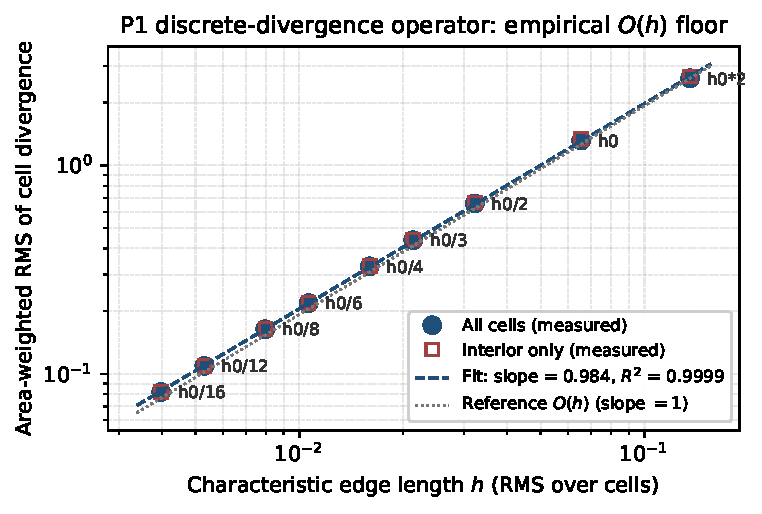
\includegraphics[width=0.82\linewidth]{figures/fig_4_operator_floor_loglog.pdf}
\caption{P1 divergence operator-floor calibration.}
\label{fig:operator-floor}
\end{figure}

\subsection{Coverage implication: fault-detection robustness across the multi-checkpoint roster}
\label{subsec:fault-robustness}

The 10-mutant catalogue is replayed against the K=6 roster with five input-permutation seeds (30 trials per mutant per detector) and predeclared severity sweeps for NS\_double\_scale and PC\_zero\_vy. Detection uses pilot thresholds: node-permutation tolerance $10^{-5}$, conservation ratio 1.5, and mirror-y relative-change 0.5. Wilson intervals are over (SUT, seed) cells. This is the primary MGN stress-test denominator, not the whole fault-evidence inventory.

Table~\ref{tab:coverage-geometry} summarizes coverage geometry: each admitted relation measures one invariant family, so blind cells are structural, not sampling noise.

\begin{table}[!htbp]
\centering
\caption{Coverage-geometry matrix.}
\label{tab:coverage-geometry}
\scriptsize
\renewcommand{\arraystretch}{0.93}
\begin{tabularx}{\linewidth}{@{}>{\raggedright\arraybackslash}p{0.18\linewidth}>{\raggedright\arraybackslash}p{0.26\linewidth}>{\raggedright\arraybackslash}p{0.26\linewidth}Y@{}}
\toprule
\textbf{Detector / relation family} & \textbf{Visible directions} & \textbf{Blind or excluded directions} & \textbf{Scope and boundary} \\
\midrule
Node permutation & Representation contract passes exactly; also admitted on airfoil & Canonical injected faults preserve node relabeling, so no mutant is detected & Sanity/adapter evidence, not fault-coverage evidence \\
Continuity / conservation & Boundary-condition faults and gross normalization faults; shared continuity $\to$ normalization-scale signal on airfoil & Multiplicative output scaling sweep remains undetected (0/6, CI $[0.00,0.39]$) & Measures conservation-like invariants only; absolute MGN conservation remains deferred \\
Mirror-y symmetry & Physical-channel and mesh-adjacency faults; partial $v_y$ zeroing detected through $p=0.99$ (6/6) & Exactly uniform $p=1.0$ is blind (0/6); mirror-y excluded on non-zero-angle airfoil & Coverage disappears when the relation is inadmissible \\
Admitted suite & 5/10 canonical MGN mutants detected; reproduces across S0--S3, with 4/10 on S4/S5 & Invariant-preserving faults remain invisible, including adversarial escapes & Bounded stress-test coverage, not real-world defect-detection rate \\
Cross-family / cross-program checks & PINN/FNO probes and sibling programs reproduce the invariant-based reading & Trained-mutant MGN/PointMLP evidence and closed-form PINN/FNO probes are not interchangeable & Breadth evidence only; no calibrated coverage law \\
\bottomrule
\end{tabularx}
\end{table}

\textbf{Aggregate reading.} The 5/10 union detection rate reproduces across S0--S3 and nearly across S4/S5. Continuity is sensitive to boundary/scale faults; mirror-y is sensitive to physical-channel and adjacency faults; invariant-preserving faults remain invisible. The 60-entry catalogue and two adversarial mutants make the blind region explicit: A1 is detected only by mirror-y, and A2 escapes every detector. On airfoil, mirror-y is excluded by non-zero angle of attack, so mirror-only cylinder-flow coverage disappears. The sibling adds breadth across seven program types and five CPU-only replays.

\textbf{Independent periodic-advection primary workflow.} The \textbf{periodic-advection primary workflow} adds an independent synthetic 2D scalar advection task with six deterministic NumPy-trained periodic-convolution SUTs and 10 held-out fields per SUT. It records relation records, checkpoints, source/follow-up outputs, ledgers, gate decisions, and verdicts. Periodic translation is admitted and gives \textbf{60/60 translation passes}; mass/mean conservation is admitted and gives \textbf{60/60 mass-conservation passes}; the \textbf{fixed-velocity mirror candidate is rejected} for 6/6 SUTs because mirroring the scalar field without transforming velocity changes the transport problem. This is full gate-to-verdict evidence on an independent synthetic PDE task, \textbf{not production CFD or real-defect evidence}.

\subsection{Interpretation and boundaries}
\label{sec:discussion}
\label{subsec:still-blocked}
\label{subsec:scoped-interpretation}

The study's value is relation-level interpretation, not universal fault finding. Retained MRs complement accuracy/UQ diagnostics, constrain fault attribution, and make assumptions inspectable; they do not license superiority, reliability, geometry-independent rates, validated localization, real-world defect rates, zero-cost MR discovery, or measured person-hour savings. Two overclaims are blocked: asymmetric-mesh mirror-y remains OOD stress, and absolute discrete-divergence is deferred rather than recorded as a conservation pass. Symmetric meshes, airfoil, PINN, and FNO show that these verdicts are not only post-hoc labels.

\textbf{Boundary of claims.}
\label{subsec:boundary-claims}

The blocked list remains active: no external-dataset or geometry-independent rates, AeroGraphNet/DoMINO results, baseline superiority, real-world defect rates, validated localization, runtime, reliability, or model-accuracy claims. The supported claim is auditable MR execution for the studied SciML SUTs.

\textbf{Implications for SciML testing.}
\label{subsec:implications}

The workflow turns implicit expert checks into explicit relation records and executable checks that complement residuals, UQ, and accuracy; cross-SUT calibration remains future work.

\textbf{When to use, and at what cost.} The gate is useful when an OOD surrogate has a physically necessary relation that can be made numerically decidable. It still requires domain, numerical, and testing expertise; effort, agreement, and maintenance cost remain unmeasured.

\section{Threats to Validity}
\label{sec:threats}

We classify threats following Verdecchia et al.~\citep{verdecchia2023threats} and report against the Empirical Standards for software engineering research~\citep{ralph2021empirical}.

\textbf{Construct validity.} The construct is admissibility-gated relation record and executable check construction, not model correctness. Wrong physics, boundary conditions, mappings, operators, or tolerances could change a verdict; each relation therefore needs a relation record, explicit preconditions, typed verdict, and floor argument. The P1 floor covers the deployed symmetric mesh and one Delaunay topology, not arbitrary meshes; conservation is a non-regression guard; seeded-fault rates do not estimate real-world prevalence.

\textbf{Internal validity.} Setup, checkpoints, seeds, preprocessing, normalization, and runtime nondeterminism may affect verdicts. Manifests, ledgers, and raw outputs are recorded; cylinder-flow checks are repeated across K=6 checkpoints, three trajectories, variants, PointMLP, and PhysicsNeMo. These repetitions reduce single-run risk but do not make cells independent samples. Airfoil is read for gate discrimination, not model accuracy.

\textbf{External validity.} Evidence spans cylinder flow, airfoil, PINN/FNO Burgers and heat runs, periodic advection, RealPDEBench, a five-unit external issue/PR/commit-linked witness corpus, and sibling cross-program checks. This weakens the self-made-task objection, but does not support general reliability, production-CFD validation, representative real-defect rates, framework-wide correctness, new MR discovery, or superiority.

\textbf{Baseline and comparator validity.} Rollout accuracy, residual/UQ diagnostics, generic templates, and LLM-assisted candidates are scope contrasts, not defeated competitors. LLM outputs depend on prompts, model versions, and simulated raters; the deterministic admissibility gate is the validity authority.

\textbf{Conclusion validity.} Counts and intervals are used only where the sampling unit supports them. Many cells share checkpoints, trajectories, or generated cases; the conclusion is bounded empirical utility for RQ4, not calibrated reliability or coverage.

\textbf{Reproducibility.} Old runtimes, public loaders, and non-redistributable inputs limit exact reruns, so the package prioritizes scripts, manifests, logs, ledgers, and available outputs. CPU replay covers floors, validators, typed verdicts, checkpoints, and ledgers; PhysicsNeMo/airfoil training needs GPU access and public DeepMind TFRecords.

\section{Future Work}
\label{sec:future-work}

Future work should extend numerical-decidability theory beyond shape-regular P1 triangles; calibrate the domain-violation axis; evaluate production-scale SUTs, independent real-defect corpora, and independently authored mutants; and automate Relation-record authoring, precondition checking, and ledger generation while measuring effort and maintenance cost.

\section{Conclusion}
\label{sec:conclusion}

This paper asked when a physics-derived MR for SciML surrogate software is sound enough to use as an oracle-free test. The answer is a numerical-decidability admissibility criterion: check physical basis, domain preconditions, representation mapping, and operator-floor dominance before execution, then record the result as a relation record, executable check, ledger entry, and typed verdict.

The evidence is bounded but artifact-backed. Cylinder-flow MeshGraphNets separate a representation pass, mirror-y OOD stress, deferred absolute conservation, and a reference-relative diagnostic; operator-floor analysis explains the deferral; airfoil, PINN, FNO, periodic-advection, and cross-program executions show that the gate changes or preserves verdicts according to relation conditions; and seeded faults expose admitted-set blind spots without implying general defect rates. The contribution is methodological: physically meaningful SciML MRs require explicit validity conditions, numerically decidable verdicts, executable checks, raw evidence, and visible claim boundaries.

\section*{Preprint}
An earlier preprint version of this manuscript is available on arXiv at \url{https://arxiv.org/abs/2606.17529} with DOI \url{https://doi.org/10.48550/arXiv.2606.17529}.

\section*{CRediT authorship contribution statement}
\textbf{Meng Li:} Conceptualization, Methodology, Software, Writing -- original draft. \textbf{Xiaohua Yang:} Supervision, Formal analysis, Writing -- review \& editing. \textbf{Jie Liu:} Investigation, Validation. \textbf{Shiyu Yan:} Data curation, Visualization.

\section*{Declaration of competing interest}
The authors declare no conflict of interest.

\section*{Declaration of generative AI and AI-assisted technologies in the writing process}
During the preparation of this work the authors used generative AI assistants for code scaffolding, prose copy-editing, and reference cross-checking. After using these tools the authors reviewed and edited the content as needed and take full responsibility for the content of the publication. No generative AI was used to fabricate, alter, or invent experimental data, results, or citations; every numerical claim is backed by a tracked artifact under \texttt{research\_assets/runs/} and a claim-ledger entry.

\section*{Acknowledgments}
This work was supported by the National Natural Science Foundation of China (NSFC) General Program (grant no.\ 12575176), the Hunan Provincial Education Department Project, China (grant no.\ 202502000728), the Natural Science Foundation of Hunan Province, China (grant no.\ 2025JJ70193), and an industry-funded research project (grant no.\ 230KHX060001).

\section*{Data availability}
The replication package is archived on Zenodo at \url{https://doi.org/10.5281/zenodo.20702952}, with source at \url{https://github.com/meng004/Domain-Validity-Gated-MR-for-SciML}. It contains the manuscript source, relation records, validators, claim ledger, run manifests, metric ledgers, and committed derived outputs under \path{research_assets/runs/}. Minimum-MR-SubSet audit/rerun artifacts cite commit \path{9ef862ec37335b4834d0a1fb38b4b613af702f34}. DeepMind cylinder-flow and airfoil TFRecords are public benchmark inputs staged by the workflow runners rather than redistributed in the manuscript package. GPU-dependent reruns and credential requirements are documented in \path{REPRODUCIBILITY.md}; absent credentials cause fail-closed precondition checks rather than silent substitution.

\section*{Supplementary material}
\label{sec:supplementary-material}
The detailed claim-to-evidence map, cross-program breadth notes, secondary baseline audit, cross-family PINN/FNO execution details, RealPDEBench foil preflight witness, and external defect-witness corpus are supplied as supplementary material. The authoritative runtime mapping remains in \texttt{research\_assets/experiments/claim-ledger.yml}; the submitted supplement preserves the extracted tables and boundary statements used to audit the manuscript claims.

\bibliographystyle{elsarticle-harv}
\bibliography{references}

\end{document}
